To be able to find the balls it is needed to understand how, using images, it is possible to differentiate between the table and the different balls. In this section the colors of the table and the different pool balls will be measured for further analysis.\\

\textbf{The table:}\\
As written in the rules\ref{sec:rules} the table cloth colour has to be yellow-green, blue-green or electric blue. The cloth color should be constant, but dependent on the lightning the variance of the cloth on the input image could be significant.

The table which has been used for measuring is a pool table with !!COLOUR!! which is located in Aalborg University's lab at !!BLABLA!!. 

Three different images of the pool table and one image with the cloth cut out are analysed first in HSV color space and then i RGB space. These analysis will be used in the solution chapter.

\begin{figure}[H]
\begin{center}
\leavevmode
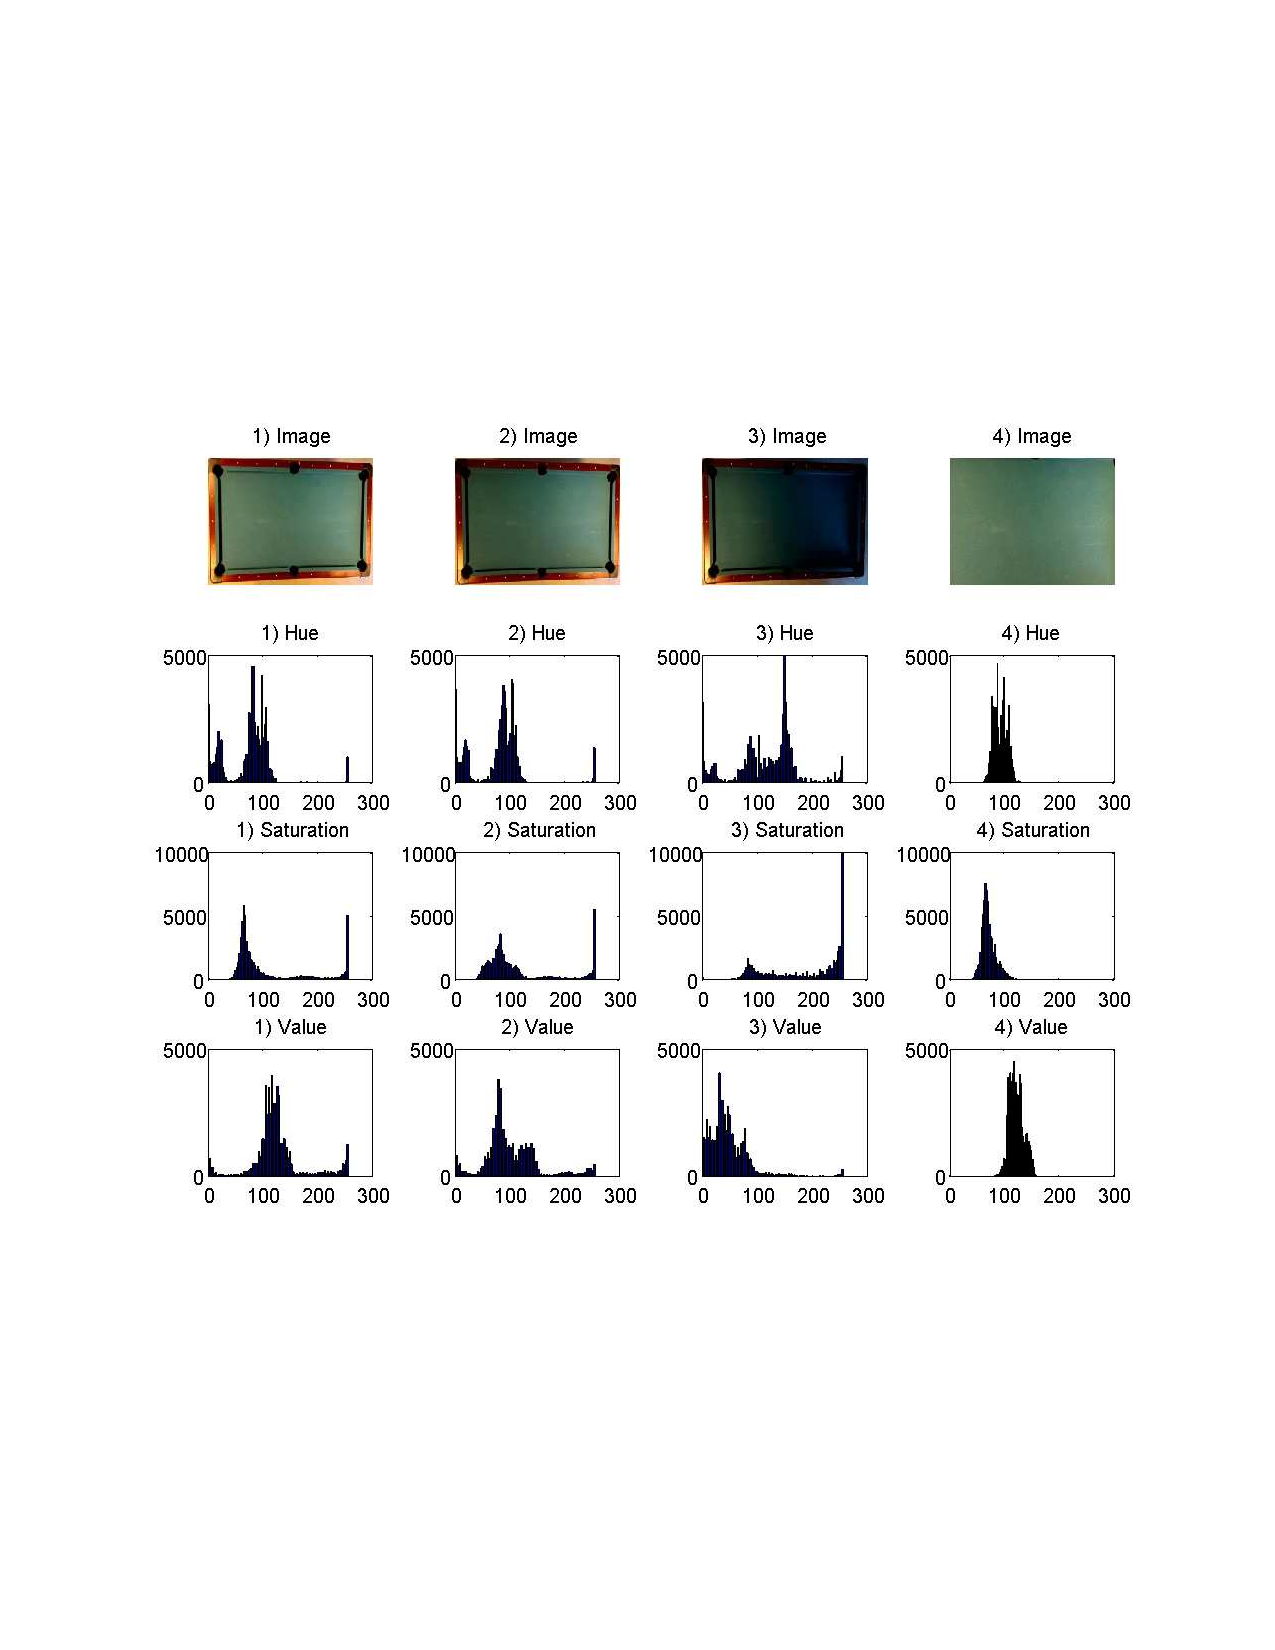
\includegraphics[width=0.9\textwidth]{images/table_hist_hsv.pdf}
\end{center}
\caption{HSV: Image 1,2 and 3 are mixed lightning where 4 is the cutout of the cloth.}
\label{fig:tablehsv}
\end{figure}

\begin{figure}[H]
\begin{center}
\leavevmode
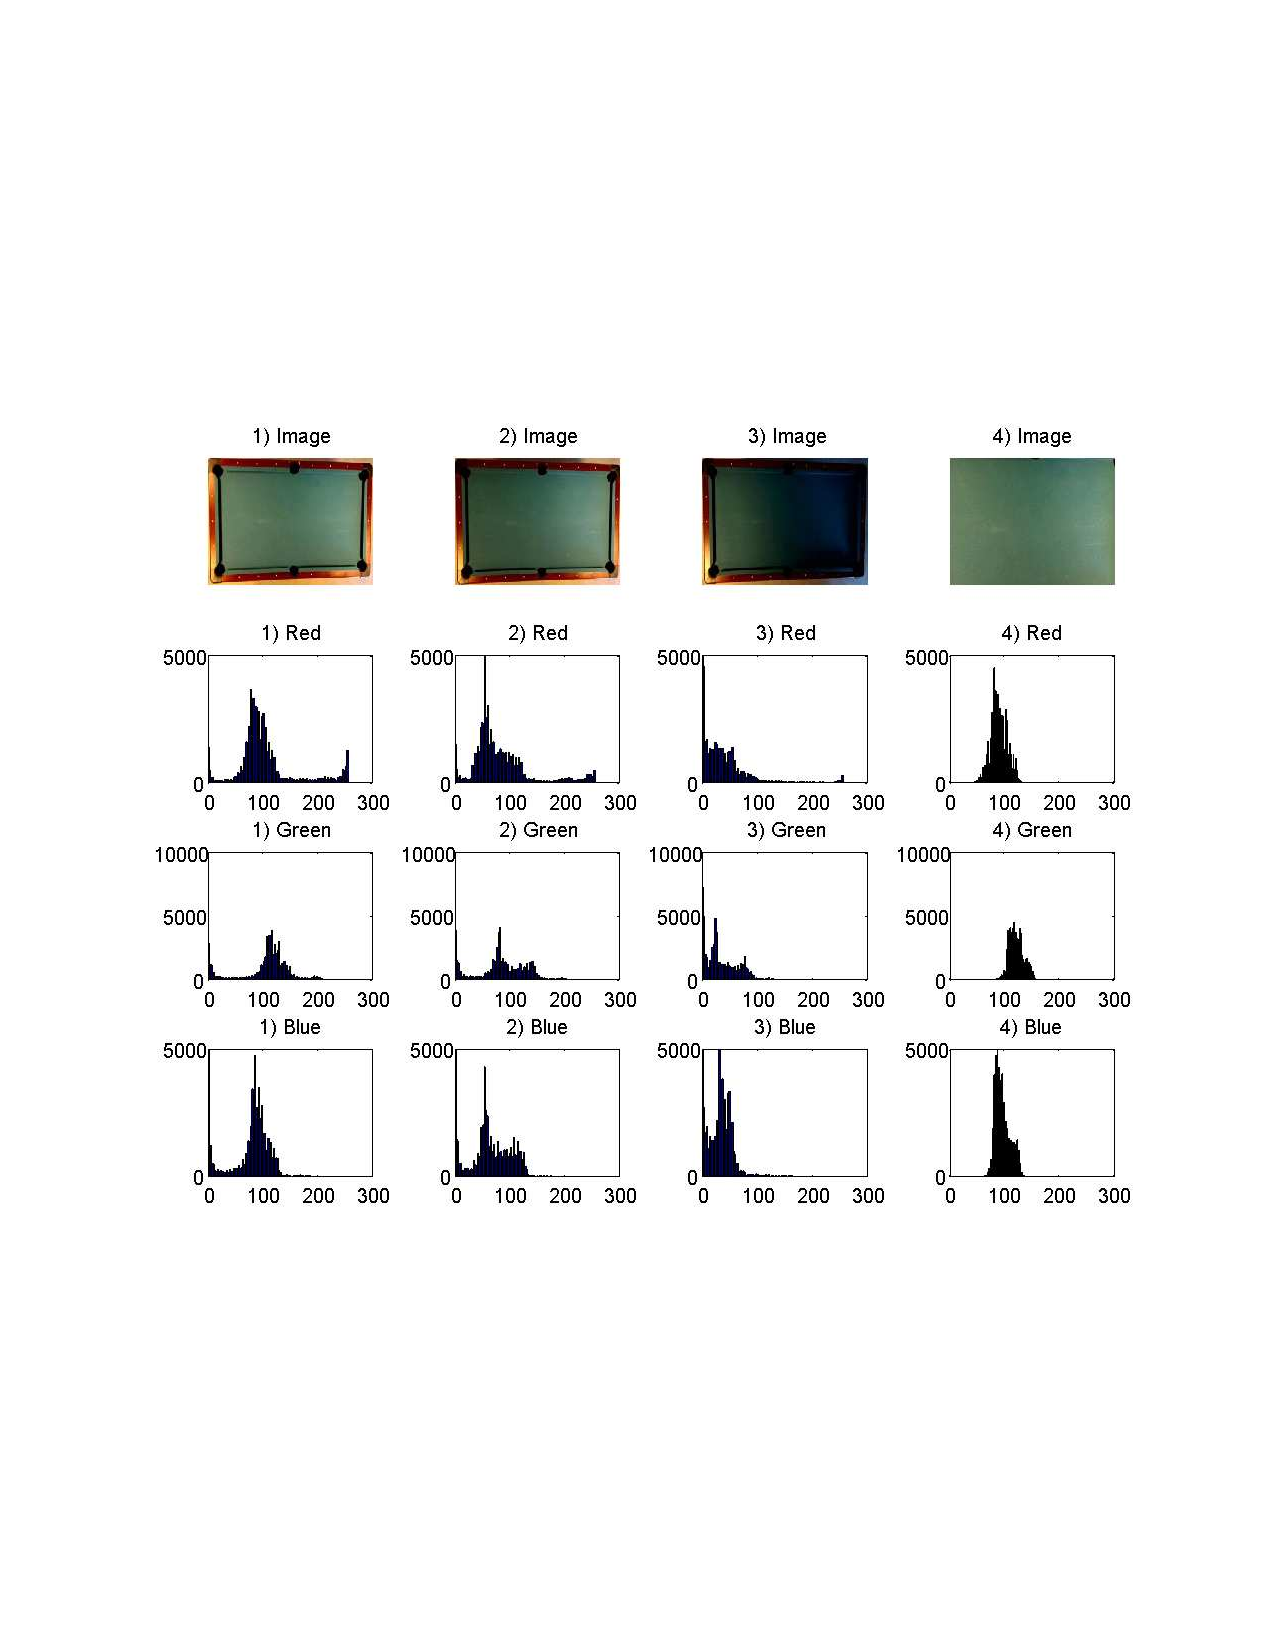
\includegraphics[width=0.9\textwidth]{images/table_hist_rgb.pdf}
\end{center}
\caption{RGB: Image 1,2 and 3 are mixed lightning where 4 is the cutout of the cloth.}
\label{fig:tablergb}
\end{figure}




\textbf{The balls:}\\